\documentclass[12pt]{article}
\usepackage{amsmath}
\usepackage{amssymb}
\usepackage{fancyhdr}
\usepackage{graphicx}
\usepackage{pdfpages}
\usepackage{listings}
\usepackage{color}
\usepackage{lmodern}
\usepackage{hyperref}

\definecolor{dkgreen}{rgb}{0,0.6,0}
\definecolor{gray}{rgb}{0.5,0.5,0.5}
\definecolor{mauve}{rgb}{0.58,0,0.82}
\pagestyle{headings}
\setlength{\oddsidemargin}{0in}
\setlength{\evensidemargin}{0in}
\setlength{\textheight}{9in}
\setlength{\textwidth}{6.5in}
\setlength{\topmargin}{-0.5in}
\setlength{\headheight}{14pt}
\renewcommand*\rmdefault{lmss}
\renewcommand*\contentsname{Table of Contents}
\lstset{language=Matlab,
	aboveskip=3mm,
	belowskip=3mm,
	showstringspaces=false,
	basicstyle={\normalfont\ttfamily},
	numbers=left,
	numberstyle=\tiny\color{gray},
	keywordstyle=\color{blue},
	commentstyle=\color{dkgreen},
	stringstyle=\color{mauve},
	breaklines=true,
	breakatwhitespace=true,
	tabsize=4
}

\newcommand{\horizontalLine}{
	\begin{center}
		\hrule width 1.0\textwidth
	\end{center}
}

\newcommand{\smallHorizontalLine}{
    \begin{center}
        \hrule width 0.5\textwidth
    \end{center}}

%%%%%%%%%%%%%%%%%%%%%%%%%%%%%%%%%%%%%%%%%%%%%%%%%%%%%%%%%%
%%%%%%%%%%%%%%%%%%%%%%%%%%%%%%%%%%%%%%%%%%%%%%%%%%%%%%%%%%
\title{\vspace{-3ex}\bf Final Project Report\\[2ex] 
       \normalsize ECS 171: Machine Learning\\Fall 2015}
\date{\today}
\author{\bf Team Name: The Muses\\ \bf William Otwell (997371020)\\ \bf Marshall Hampson (998795016)\\ \bf Nicholas Layton (996933702)\\ \bf Steven Mackey ()\\ \bf James Dryden (993083613)\\ \bf Amos Too (998124687)\\ \bf Michael Fiueroa (998378271)\\ \bf Peggy Li (998440170)}

%%%%%%%%%%%%%%%%%%%%%%%%%%%%%%%%%%%%%%%%%%%%%%%%%%%%%%%%%%
%%%%%%%%%%%%%%%%%%%%%%%%%%%%%%%%%%%%%%%%%%%%%%%%%%%%%%%%%%
\begin{document}
\maketitle
\pagebreak
\tableofcontents
\pagebreak

%%%%%%%%%%%%%%%%%%%%%%%%%%%%%%%%%%%%%%%%%%%%%%%%%%%%%%%%%%
%%%%%%%%%%%%%%%%%%%%%%%%%%%%%%%%%%%%%%%%%%%%%%%%%%%%%%%%%%
\section{Abstract}
\label{sec:abstract}
Music lovers worldwide are in constant search of new sounds to enrich their music library. Many analytic applications have risen to popularity as a result of listeners' need for music discovery. Most of these applications utilize machine learning techniques to make recommendations and predictions for their users. One of the more common problems in music analytics is the process of recommending an enjoyable song or artist to a user based on their previous music choices. Another popular problem is the process of generating a personalized playlist for a user, again based on their listening choices. 

We sought to solve similar problems by performing predictive analytics on songs based on their acoustic qualities. We hoped to discover any relationship between a song's acoustic qualities and its inaudible qualities, such as genre or popularity. Ultimately, we constructed models to perform different types of analysis, depending on the complexity and structure of the problems. 

%%%%%%%%%%%%%%%%%%%%%%%%%%%%%%%%%%%%%%%%%%%%%%%%%%%%%%%%%%
%%%%%%%%%%%%%%%%%%%%%%%%%%%%%%%%%%%%%%%%%%%%%%%%%%%%%%%%%%
\horizontalLine
\section{Introduction}
\label{sec:introduction}

\subsection{Background}
\label{subsec:background}
The motivation to develop "smarter" software for music analytics originates largely from a desire to sell more products to customers. Some of the biggest players in the industry, Amazon and Apple, are notoriously known for their "genius" recommendations on what customers ought to buy next. Brian Whitman, co-founder and CTO of the Echo Nest, said in his article titled \textit{How music recommendation works - and doesn't work} that, "Amazon is not optimizing for the noble work of raising independent artists' profiles to the public, and they're definitely not optimizing for a good musical experience. They're statistically optimizing to make more money, to sell you more things." Brian also discusses how many radio companies, like Pandora, utilize popularity to provide an enjoyable radio-listening experience. Although many of these companies have found success using their own techniques, Brian ultimately expresses the importance of not only focusing on these money-making techniques but satisfying listeners by focusing on the actual music, its sound waves and lyrical significance. He believes that the sound of a song can contribute much more to predictive analytics than users' purchase history or song popularity.

Our approach to music analytics was similar to that of Brian Whitman's company, minus the lyrical analysis. We utilized data that represented the actual sound of the music, an approach that Brian calls "acoustic analysis." Some of the features that we included in our analysis, for example, were time signature, loudness, and key, to name a few. We hoped to focus our analysis on the sounds of the music and how the features of a song itself could provide predictive information. More specifically, the goals we hoped to accomplish were:
\vspace{-3.5mm}
\begin{itemize}
    \item Predict the popularity of a song by applying linear regression techniques to quantify and predict the popularity of a song based on its acoustic features
    \vspace{-3.5mm}
    \item Classify a song into its genre(s) by utilizing artificial neural networks to learn about the potential relationship between a song's acoustic qualities and its associated genres 
    \vspace{-3.5mm}
    \item Discover trends in the songs regarding hotness and genre by utilizing clustering techniques to discover trends in a songs features that might indicate a songs "hotness"
    \vspace{-3.5mm}
\end{itemize}

\subsection{Million Song Dataset}
\label{subsec:datasetIntro}
The dataset that we chose to use is known as the Million Song Dataset (see Appendix~\ref{subsec:datasetsAndCode} for more info). Rather than actually using 1 million songs, we used a small, manageable subset of the Million Song Dataset. The features that we used were: danceability, duration, end-of-fade-in, energy, key, loudness, mode, song-hotness, start-of-fade-out, tempo, time-signature, year, and artist-terms, which is simply a list of tags (which in our case can be thought of as genres) for each song.

%%%%%%%%%%%%%%%%%%%%%%%%%%%%%%%%%%%%%%%%%%%%%%%%%%%%%%%%%%
%%%%%%%%%%%%%%%%%%%%%%%%%%%%%%%%%%%%%%%%%%%%%%%%%%%%%%%%%%
\horizontalLine
\section{Methods}
\label{sec:methods}

%%%%%%%%%%%%%%%%%%%%%%%%%%%%%%%%%%%%%%%%%%%%%%%%%%%%%%%%%%
\subsection{Linear Regression: Song Popularity}
\label{subsec:linearRegression}
In an effort to study the predictability of song "hotness" (a measure of popularity included in our data), we used linear regression and various feature sets to create a working model. We began with feature reduction, using Lasso regression and Pricipal Component Analyses followed by normal linear regression. We began modeling with the above listed features, but with danceability and energy ignored. We also selectively used elements with a listed hotness of zero. Such an absolute value suggests missing data more than complete dearth of popularity, so we removed it in some models. This greatly reduced the resulting error. We also tested the use of different numbers of song tags. Using a list sorted by number of appearances in the data, we examined the effects of using the top 20 elements vs just the top 5. We represented these song tags as a matrix in which the rows are associated with sample and the columns with the different song tags. Every $m \times n$ element in the matrix contains a binary value representing the presence or absence of the corresponding song tag in the data pertaining to that row element.

We found that the overwhelmingly important factors in creating an accurate model were the presence and number of song tags, and avoiding overfitting with more complicated feature reduction techniques. The highest mean squared error we found was when we used Lasso regression, followed by our PCA driven attempt. In the end our best result came from retaining a modest number of song tags (20), using normal linear regression, and removing elements with missing or zero valued hotness.

%%%%%%%%%%%%%%%%%%%%%%%%%%%%%%%%%%%%%%%%%%%%%%%%%%%%%%%%%%%%%
\subsection{Artificial Neural Networks: Song Genres}
\label{subsec:ann}
We utilized Neural Networks to predict song genres based on features of a song. Many songs, however, belonged to several genres. To represent the various genres, also known as tags, for a particular song, we formed a feature column for each possible tag in our dataset. Then, we scanned through each song to determine its set of tags and set the index of each tag to a 1 in the appropriate column if the tag was present for the particular song. If there were $n$ possible tags in the entire dataset, and $m$ samples, then the matrix needed to represent all tags for all samples would be an $m \times n$ matrix. Ultimately, our data matrix looked something like this:
\begin{equation}
    X = \begin{Bmatrix}
    	x^{(1)}_1 & x^{(1)}_2 & ... & x^{(1)}_{n_1} \\
    	...       & ...       & ... & ... \\
        x^{(m)}_1 & x^{(m)}_2 & ... & x^{(m)}_{n_1} \\
    \end{Bmatrix},
    \\
    Y = \begin{Bmatrix}
    y^{(1)}_1 & y^{(1)}_2 & ... & y^{(1)}_{n_2} \\
    ...       & ...       & ... & ... \\
    y^{(m)}_1 & y^{(m)}_2 & ... & y^{(m)}_{n_2} \\
    \end{Bmatrix},
    \\
    D = \{X,Y\}
\end{equation} 
\begin{equation}
    x^{(i)}_j \in \Re\ \text{and}\ y^{(i)}_j \in \{0, 1\}
\end{equation}

where $n_1$ is the number of features, $n_2$ is the number possible tags, and $m$ is the number of samples.

We quickly found that if we included all of the possible tags from our dataset that the number of tags would reach an unmanageable amount. Training our network with such a large number of tags was computationally intensive and was difficult for our network to learn such a complex distribution. Instead, we decided to limit the number of tags to a small subset of the most popular tags. We were able to import a list of the 300 most popular genres in the dataset and use it as the limiting set of possible tags for our dataset. We found that even 300 tags was too many. Later, we found that limiting the possible number of tags would reduce error and misclassification rate.

By having 12 song features and $n_2$ possible genres, we knew we would need to construct a neural network with 12 input nodes and $n_2$ output nodes. The more complicated issue arose when we tried determining the adequate number of hidden nodes.

We were mostly interested in observing the effect of 3 different parameters on the neural network: learning rate, number of hidden layers, and number of hidden nodes per hidden layer. We planned on running our dataset through various neural networks, each with a different configuration of the above parameters. We hoped to find an optimal configuration for these parameters while also discovering any correlation between the above song features and the song tags. A particular configuration of these parameters that yielded both minimal training error and misclassification rate would implicitly verify a correlation between song features and song tags.

%%%%%%%%%%%%%%%%%%%%%%%%%%%%%%%%%%%%%%%%%%%%%%%%%%%%%%%
\subsection{Clustering: Hotness}
\label{subsec:clustering}
We took two different approaches to clustering our data: k-means and hierarchical. We looked at k-means to try and see if there had any obvious patterns and then see if those patterns held any significance for genre or song hotness. The hierarchical approach is intended to give us insight to the distribution of our data and help us select the appropriate number of clusters for k-means. For both approaches we chose to use MATLAB and take advantage of the built-in clustering methods.

For K means and hierachical, we used the subset of data mentioned previously. We noticed that danceability and energy where all 0 in the provided dataset although the value was supposed to range between 0 and 1. Therefore we decided to not use these features in our clustering. We also removed year and mode because the ended up being nearly categorical: their normalized values were almost 0 or almost 1. Finally, We also only used the samples that had a value for hotness as many were set to 0 indicating no data. 

For k-means clustering we ran our reduced data through the MATLAB k-means function and plotted of all these features plotted against song hotness. We started with a guidline to use sqrt(n/2) clusters. We ran k-means using this guidline, producing 44 clusters. We tried using various other numbers of clusters and decided to display results using only 4 clusters.

To get the hierarchical clusters and plot the dendrogram we used the MATLAB functions dendrogram and linkage. The linkage function returns a tree of when to clusters are linked together. We decided to view the dendrogram with at most 50 distinct clusters. We compared this to a dendrogram of random data.

%%%%%%%%%%%%%%%%%%%%%%%%%%%%%%%%%%%%%%%%%%%%%%%%%%%%%%%%%%
%%%%%%%%%%%%%%%%%%%%%%%%%%%%%%%%%%%%%%%%%%%%%%%%%%%%%%%%%%
\horizontalLine
\section{Results}
\label{sec:results}

%%%%%%%%%%%%%%%%%%%%%%%%%%%%%%%%%%%%%%%%%%%%%%%%%%%%%%%%%%
\subsection{Linear Regression}
\label{subsec:linearRegressionResults}
The feature sets we elected to work with were a combination of the original data set, subsets of the song tags data field, and some attempts at cleaning up the elements used in training. The first thing we tried was feature selection using Lasso regression and all features and all song tags. The resulting MSE was the highest of all trials: 0.25. The next feature reduction strategy we used was Principal Component Analyses with a second highest error of 0.0488. Looking at the scatter plot of predicted vs actual values, we see two clear aggregated bands of points. These two bands show up in normal linear regression using all features as well, but not so neatly packed together.

Our following trials involved testing the number of song tags to include as features. We found a sorted list of the most prevalent tags in the data and modeled using 20 or 5 of them. The results here were very close, though using 20 did come out slightly more accurate in ten fold cross validation. All our tests that did not include song tags had a MSE close to 0.04, while those that did include song tags hovered closer to 0.02. The final thing we tried was to eliminate row elements with a hotness rating of 0.0. This showed measurable improvement. In the final model we used the original feature set (excluding danceability and energy as these values were all zero), the top 20 song tags, and no zero valued elements. The resulting MSE was 0.0223.

We can see the relative errors of the different models in the bar graph. On the left we see the MSE with Lasso regression. The next three are the errors associated with normal linear regression with song tags included. The lower two are corrected for zero values. The three on the right are associated with no song tags (see Appendix~\ref{subsec:MSE}).

%%%%%%%%%%%%%%%%%%%%%%%%%%%%%%%%%%%%%%%%%%%%%%%%%%%%%%%%%%%%%
\subsection{Artificial Neural Networks}
\label{subsec:annResults}
We found that the number of output nodes negatively impacted our experimental results. As mentioned before in Section~\ref{subsec:ann}, we found that limiting the number of possible genres improved both the training error and misclassification rate. Initially, we constructed our network with 12 input nodes and $n_2 = 301$ output nodes. We then attempted to iterate through various configurations of hidden layers, hidden nodes, and learning rates, but found that none of them yielded results anywhere remotely near desirable.

After considering our options for improving the performance of our network, we limited the maximum number of output nodes to $n_2 = 5$. For each sample we only took genres that belonged to the top 5 genres from our list of most popular genres. The top 5 genres were: rock, electronic, pop, alternative rock, and hip hop. Songs that didn't belong to any of these genres would ideally not be classified into any category. Graphs from our revised network configurations can be found in Appendix~\ref{subsec:annBetterPerformance}.

Ultimately, we found that the lowest number of output nodes would yield the most optimal results. We chose to limit the output nodes to only the most popular genre: rock. It was no surprise that this configuration would yield the most optimal results since the network needed only to focus on a single output node. Once we discovered that this output-node configuration was the best, we ran the loop that is shown in Appendix~\ref{subsec:annLoop} to discover the optimal hidden-layer and learning rate configuration. The results of this loop are shown in Appendix~\ref{subsec:variousANN}, which is a plot of the minimum of both the training error and misclassification rate for each network configuration. From this plot, we see that the optimal configuration is the 7th network: 4 hidden layers, each with 12 hidden nodes, with a learning rate of 0.05. A plot of the training run for this network is shown in Appendix~\ref{subsec:annBestPerformance}.


%%%%%%%%%%%%%%%%%%%%%%%%%%%%%%%%%%%%%%%%%%%%%%%%%%
\subsection{Clustering}
\label{subsec:clusteringResults}
We found that the clusters seemed to be skewed by issues with our data set. Plotting our data before removing year and mode skewed our data into clusters based only on these two features. Before removing the bad from hotness, our clusters were all significantly shifted towards zero hotness. However, our data did not split into zero hotness clusters vs non zero hotness clusters. All the clusters were shifted down equally. After removing these features and a set of incomplete elements from the dataset, we found we got more distinct clusters. Below is our k-means clustering with four clusters, both before and after removing features.

%INSERT DIAGRAM: trimmed & untrimmed 

We compared our hierarchical dendrogram to that of a randomly generated sample. They showed a very similar structure. Comparing the distance values from the dendrograms, we found that there were really 4 distinct leaves in our data. After the 4 initial splits, future splits didn't look any more significant than they would in a dendrogram for random data. Below are the dendragrams from our data and one of random data.

%INSTER DIAGRAM: random and sample dendrograms


%%%%%%%%%%%%%%%%%%%%%%%%%%%%%%%%%%%%%%%%%%%%%%%%%%%%%%%%%%
%%%%%%%%%%%%%%%%%%%%%%%%%%%%%%%%%%%%%%%%%%%%%%%%%%%%%%%%%%  
\section{Discussion}
\label{sec:discussion}

%%%%%%%%%%%%%%%%%%%%%%%%%%%%%%%%%%%%%%%%%%%%%%%%%%
\subsection{Linear Regression}
\label{subsec:linearRegressionDisc}
The likely reason for the higher error with feature reduction is overfitting. We can clearly see in the figure that PCA attempts to fit very noisy and varied data to a specific distribution (see Appendix~\ref{subsec:overfitting}, where blue are predicted and red are actual). We can see this in the scatter plot of actual vs predicted hotness. But even this result leads to suprisingly accurate predictions, with a MSE of 0.05, when hotness only ranges bewteen 0 and 1. Using normal linear regression with all the terms first-order yields an MSE of 0.02.  Also, the MSE may be a bit misleading: The mean absolute error would be around 0.15. 

Doing the same regression on groups that are split up by genre proved useful: The weights show that a popular indie rock song is much louder than a popular ambient song, for example. They also show that different genres correlate with different keys, or in higher popularity. One of the highest weighted terms in the data (over ten times the weight of other features in some cases), for example, was the first song tag: rock. Our model highly favors rock music in its prediction of the popularity of a song.
%%%%%%%%%%%%%%%%%%%%%%%%%%%%%%%%%%%%%%%%%%%%%%%%%%
\subsection{Artificial Neural Networks}
\label{subsec:annDisc}
The primary obstacle in successfully constructing a predictor for song genres was the number of genres that our network was trying to simultaneously predict. As stated in Section~\ref{subsec:annResults}, we had to reduce the number of genres from 300 to 5, and from 5 to 1 in order to get acceptable training errors and misclassification rates. The biggest problem was simultaneously reducing both the training error and the misclassification rate. 

In many of the cases, we were able to reduce the training error but weren't able to reduce the misclassification rate. We think this because of the manner in which the DeepLearningToolbox (see Appendix~\ref{subsec:datasetsAndCode} for more info about the toolbox) interprets a misclassification. Consider the case where we are trying to predict all 300 of the top genres. We would have our dataset in the configuration shown in Section~\ref{subsec:ann}, where $n_1 = 12$ and $n_2 = 300$. This results in an ANN of 12 inputs, and 300 outputs. 

Now, consider the situation in which our network correctly classifies 299 of the 300 genres, but misclassifies 1 of the genres. This situation would result in an overall misclassification by the network, even though it only missed 1 of the outputs. This makes it very easy for the network to misclassify a sample. By reducing the number of outputs to 5 and to 1, the network has a much lower possibility of misclassifying any of the particular outputs. 

It could either be that the input features don't correlate to the genres well enough to simultaneously predict them all at once, or the complexity of a neural network with 300 output nodes is just too great to handle. One of the options that we did not test that we think could help with classifying 300 outputs would be to construct a NN to handle each of the outputs, rather than having 1 NN to handle all outputs. 

%%%%%%%%%%%%%%%%%%%%%%%%%%%%%%%%%%%%%%%%%%%%%%%%%%
\subsection{Clustering}
\label{subsec:clusteringDisc}
By examining how our data clustered we hoped to find some hint as to what features were the most significant in predicting the genre or hotness of a song.
However, after examining the visualizations of the clusters there was not much to be gained by clustering. There were no obvious relationships between
the features and genre or song hotness when we used k-means to cluster the data. Hierarchical clustering seemed to reveal slightly more; at least, it was slightly more significant than hierarchical clustering on random data. This led us to conclude that using these features were not a good choice for 
determining a songs genre. 

After we realized that this didn't yield any useful information about a songs genre, we wondered what would. In the paper, "Pandoras Music
Recommender", it seems even Pandora was not able to classify music entirely by looking at features that could be calculated from audio data like in 
our approach. Rather Pandora employees a team of musicians to "[listen to a] collection of songs and tagging each according to
approximately 400 musical attributes" (Howe 2). However, they do employ clustering algorithms in order to create groups of users with certain preferences and
to cluster songs based on similarity of the human-provided tags.
So essentially, Pandora still relies on humans analyzing what genre and musical attributes have in common, but takes advantage of machine learning techniques
to predict the next song to play, by calculating the musical "distance" between songs as well as grouping users together to generate better song predictions.
%%%%%%%%%%%%%%%%%%%%%%%%%%%%%%%%%%%%%%%%%%%%%%%%%%%%%%%%%%
%%%%%%%%%%%%%%%%%%%%%%%%%%%%%%%%%%%%%%%%%%%%%%%%%%%%%%%%%%
\horizontalLine
\section{Conclusion}
\label{sec:conclusion}

We set out to discuss modeling strategies and prediction techniques in commercial music. To create a reliable and accurate model would create opportunities not only for retailers and web radio, but for artists and consumers as well. Artists could better tailor their music to their audience, and consumers would have an accurate and helpful way of finding music similar to their interests. What we found, however, is that this task is not only characterized by a large and complicated feature set, but also very prone to randomness and noise. As the models become more complicated, the computation becomes limiting and the results often do not improve (or in some cases worsen).

Furthering this study would require the addition of big data capability and an ever changing model of current trends in music. Using a combination of proper feature selection based on current popularity and a database of purchase information, we could construct a more complicated and accurate model. Among the trends that we discovered were the importance of popular genres (as our ANN group found with the rock genre) and the danger of overfitting based on poor feature selection (as or linear regression group found with PCA). In future related work we will know how to properly avoid these pitfalls.

%%%%%%%%%%%%%%%%%%%%%%%%%%%%%%%%%%%%%%%%%%%%%%%%%%%%%%%%%%
%%%%%%%%%%%%%%%%%%%%%%%%%%%%%%%%%%%%%%%%%%%%%%%%%%%%%%%%%%
\horizontalLine
\section{References}
\label{sec:references}

\subsection{Readings}
\label{subsec:readings}
\begin{enumerate}
    \item Howe, Michael. "Pandora's Music Recommender." Computer Science and Engineering. University of Washington. Web. $<$\href{http://courses.cs.washington.edu/courses/csep521/07wi/prj/michael.pdf}{http://courses.cs.washington.edu/courses/csep521/07wi/prj/michael.pdf}$>$.\vspace{-1ex}
    
    \item Whitman, Brian. "How Music Recommendation Works - and Doesn't Work." Brian Whitman. Web. $<$\href{http://notes.variogr.am/post/37675885491/how-music-recommendation-works-and-doesnt-work}{http://notes.variogr.am/post/37675885491/how-music-recommendation-works-and-doesnt-work}$>$.\vspace{-1ex}

    \item Glaser, W.T, T.B. Westergren, J.P. Stearns, and J.M. Kraft. "Consumer Item Matching Method and System." Google Books. Google Patents, 21 Feb. 2006. Web. $<$\href{http://www.google.com/patents/US7003515?dq=7,003,515}{http://www.google.com/patents/US7003515?dq=7,003,515}$>$.\vspace{-1ex}
    
    \item Visalakshi, N. Karthikeyani, and K. Thangavel. "Impact of Normalization in Distributed K-Means Clustering." International Journal of Soft Computing. Medwell Journals, 2009. Web. $<$\href{http://www.medwelljournals.com/fulltext/?doi=ijscomp.2009.168.172}{http://www.medwelljournals.com/fulltext/?doi=ijscomp.2009.168.172}$>$.\vspace{-1ex}
    
    \item Bergstra, James, Michael Mandel, and Douglas Eck. "SCALABLE GENRE AND TAG PREDICTION WITH SPECTRAL COVARIANCE." ISMIR 2010 Utrecht: International Society for Music Information Retrieval Conference. International Society for Music Information Retrieval Conference. Web. $<$\href{http://ismir2010.ismir.net/proceedings/ismir2010-86.pdf}{http://ismir2010.ismir.net/proceedings/ismir2010-86.pdf}$>$.\vspace{-1ex}
    
    \item Miotto, Riccardo, Luke Barrington, and Gert Lanckriet. "IMPROVING AUTO-TAGGING BY MODELING SEMANTIC CO-OCCURRENCES." ISMIR 2010 Utrecht: International Society for Music Information Retrieval Conference. International Society for Music Information Retrieval Conference. Web. $<$\href{http://ismir2010.ismir.net/proceedings/ismir2010-51.pdf}{http://ismir2010.ismir.net/proceedings/ismir2010-51.pdf}$>$.\vspace{-1ex}
    
    \item Serra, Joan, Alvaro Corral, Marian Boguna, and Martin Haro. "Measuring the Evolution of Contemporary Western Popular Music." Nature.com: Scientific Reports. Nature Publishing Group. Web. $<$\href{http://www.nature.com/articles/srep00521}{http://www.nature.com/articles/srep00521}$>$.\vspace{-1ex}
    
    \item Ni, Yizhao, Raul Santos-Rodriguez, Matt Mcvicar, and Tijl De Bie. "Hit Song Science Once Again a Science?" Research Homepage - Tijl De Bie. Tijl De Bie. Web. $<$\href{http://www.tijldebie.net/system/files/MML2011-final.pdf}{http://www.tijldebie.net/system/files/MML2011-final.pdf}$>$.

\end{enumerate}
\subsection{Datasets and Code}
\label{subsec:datasetsAndCode}
\href{http://labrosa.ee.columbia.edu/millionsong/}{\textbf{Million Song Dataset}}

Thierry Bertin-Mahieux, Daniel P.W. Ellis, Brian Whitman, and Paul Lamere. 
The Million Song Dataset. In Proceedings of the 12th International Society
for Music Information Retrieval Conference (ISMIR 2011), 2011.
\\
\\
\href{https://github.com/rasmusbergpalm/DeepLearnToolbox}{\textbf{DeepLearningToolbox}} - Rasmus Berg Palm

Used for the construction, configuration, training, and testing of our Artificial Neural Networks. The training algorithm uses a form of Batch Gradient Descent by constructing "mini-batches" at each iteration of training.

\appendix

%%%%%%%%%%%%%%%%%%%%%%%%%%%%%%%%%%%%%%%%%%%%%%%%%%%%%%%%%%
%%%%%%%%%%%%%%%%%%%%%%%%%%%%%%%%%%%%%%%%%%%%%%%%%%%%%%%%%%
\horizontalLine
\section{Figures}
\label{sec:figures}

\subsection{Performance of Linear Regression Models}
\label{subsec:MSE}
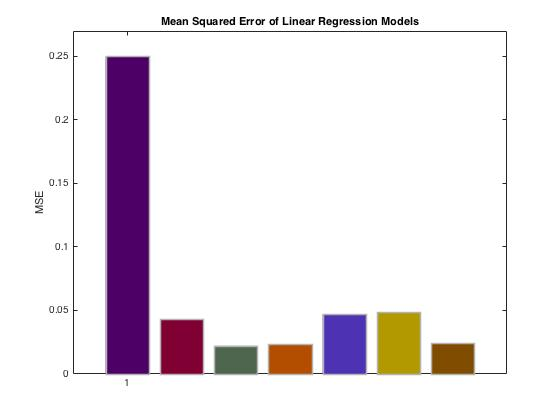
\includegraphics[scale=.5]{images/lr/mse}

\subsection{Evidence of Overfitting in Linear Regression}
\label{subsec:overfitting}
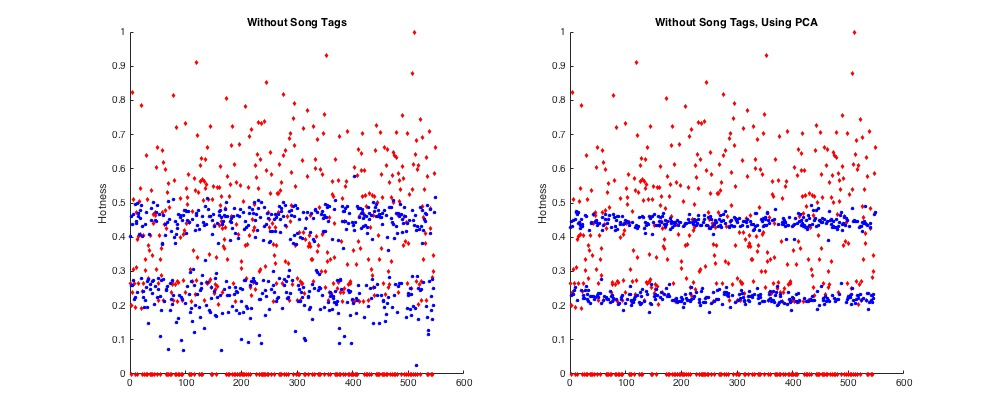
\includegraphics[scale=.4]{images/lr/overfit}

\subsection{Performance of Neural Network: 5 Output Nodes}
\label{subsec:annBetterPerformance}
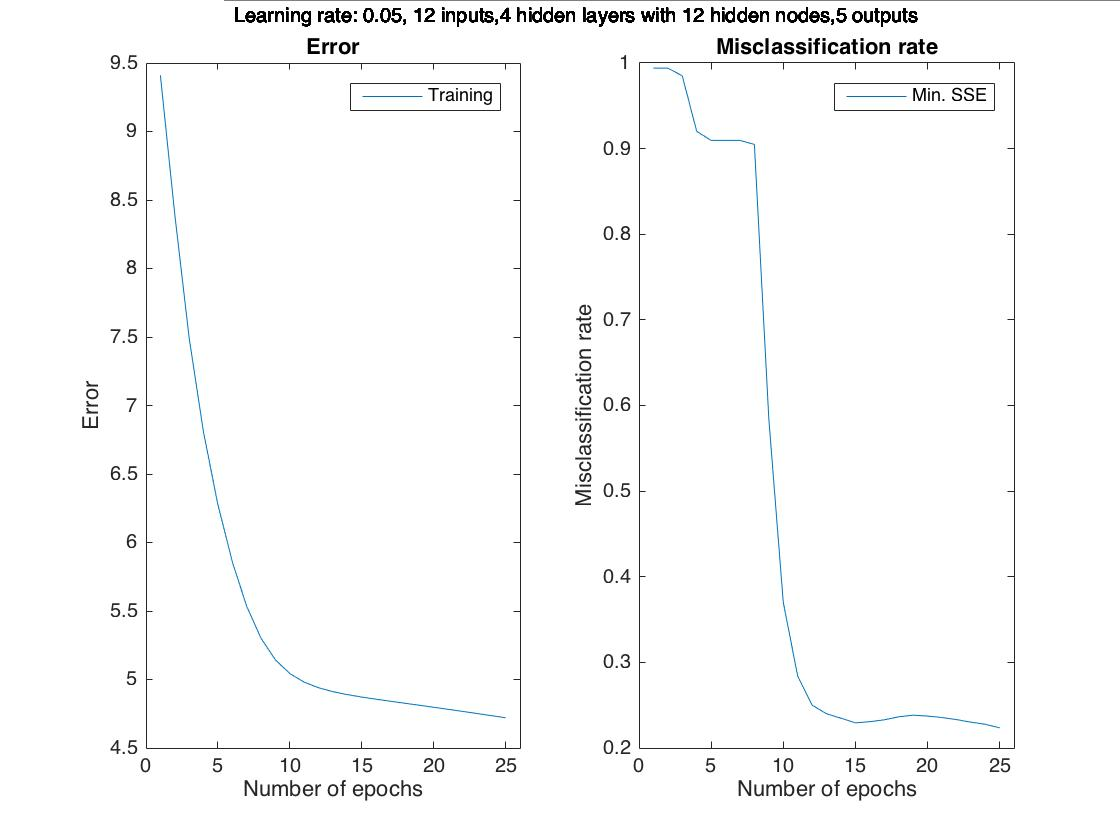
\includegraphics[scale=0.3]{images/ann/slightlyBetterWithTop5Genres2}

\subsection{Comparison of Various Neural Network Configurations}
\label{subsec:variousANN}
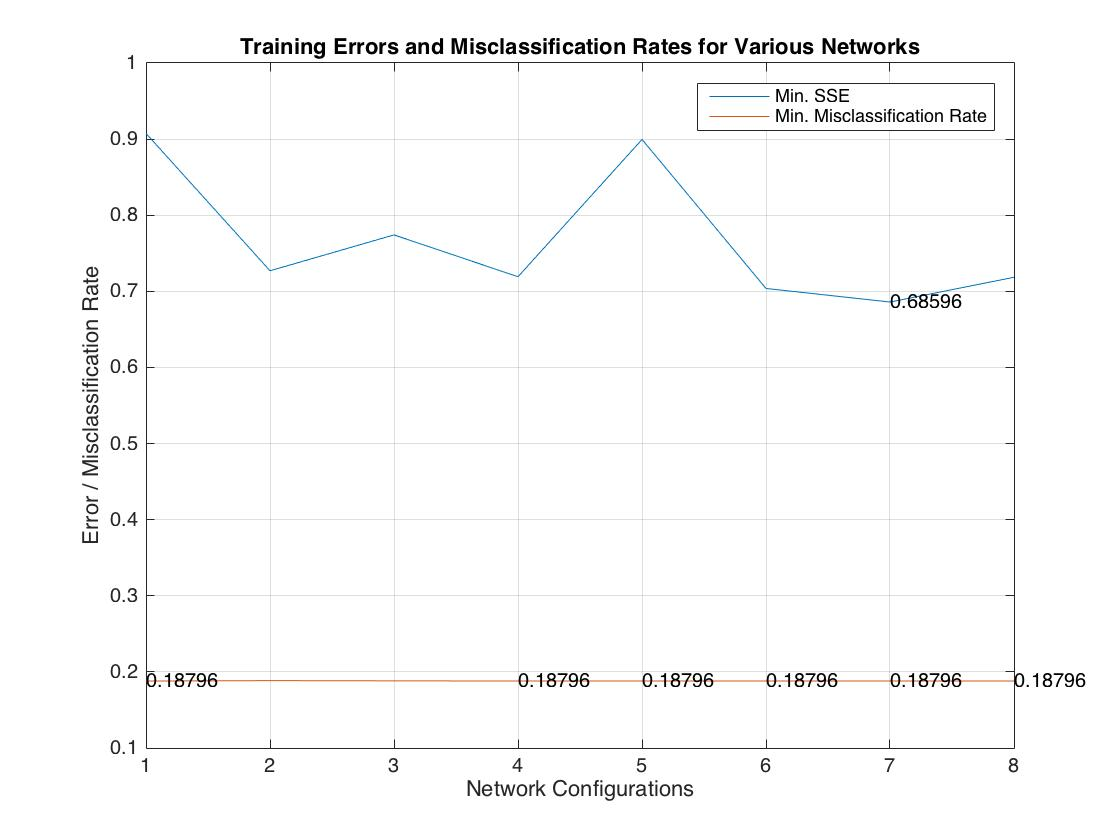
\includegraphics[scale=0.3]{images/ann/graphOfVariousNetworksWith1Genre}
\\
Each of the networks that were tested to yield the graph above contained 12 input nodes and a single output node for the classification of rock songs. The first four networks above contained 3 hidden layers, while the others contained 4. Also, the first, second, fifth, and sixth networks contained 9 hidden nodes, while the others contained 12. Finally, all of the even-numbered networks used a learning rate of 0.05, while the others used a rate of 0.1.

\subsection{Performance of Neural Network: 1 Output Node}
\label{subsec:annBestPerformance}
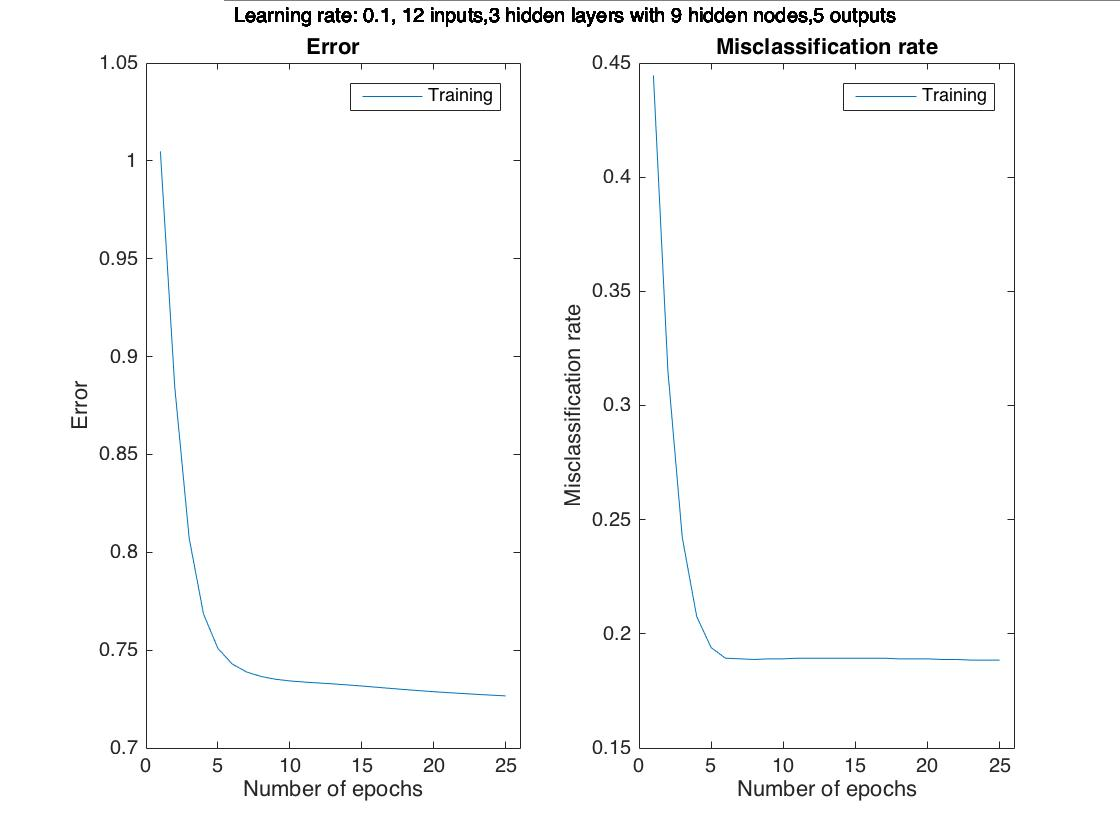
\includegraphics[scale=0.3]{images/ann/bestRun}

%%%%%%%%%%%%%%%%%%%%%%%%%%%%%%%%%%%%%%%%%%%%%%%%%%%%%%%%%%
%%%%%%%%%%%%%%%%%%%%%%%%%%%%%%%%%%%%%%%%%%%%%%%%%%%%%%%%%%
\horizontalLine
\section{Author Contributions}
\label{sec:authorContributions}
\begin{itemize}
    \item Methods:
    \begin{itemize}
        \item Linear Regression: Peggy Li, Steven Mackey, James Dryden
        \item Artificial Neural Networks: Nicholas Layton, Michael Fiueroa
        \item K-Means Clustering: William Otwell, Marshall Hampson, Amos Too
    \end{itemize}
\end{itemize}
\end{document}

